\documentclass[10pt]{article}
\usepackage[a4paper,left=0.56in,right=0.56in,top=0.48in,bottom=0.34in,footskip=10pt]{geometry}
\usepackage[T1]{fontenc}
\usepackage[utf8]{inputenc}
\usepackage{lmodern}
\usepackage{amsmath,amssymb,mathtools}
\usepackage[table]{xcolor}
\usepackage{array,booktabs,longtable}
\usepackage{multicol}
\usepackage{graphicx}
\usepackage{microtype}
\usepackage{fancyhdr}
\usepackage[hidelinks]{hyperref}
\newcommand{\OPHPaperReleaseID}{r1520}
\newcommand{\OPHPaperReleaseDate}{July 9, 2026}
\newcommand{\OPHPaperReleaseBanner}{%
\begin{center}
\small\textbf{Paper release:} \texttt{\OPHPaperReleaseID}\quad\textbf{Released:} \OPHPaperReleaseDate
\end{center}
}


\definecolor{pragmaBg}{HTML}{FFFFFF}
\definecolor{pragmaPanelTwo}{HTML}{EAF2F5}
\definecolor{pragmaInk}{HTML}{040609}
\definecolor{pragmaCyan}{HTML}{2B8997}
\definecolor{pragmaCyanText}{HTML}{095766}
\definecolor{pragmaMuted}{HTML}{5F6B7A}
\definecolor{pragmaLine}{HTML}{AFCFD8}
\definecolor{pragmaSoft}{HTML}{F1F6F8}

\pagestyle{fancy}
\fancyhf{}
\fancyfoot[C]{\footnotesize\color{pragmaMuted}\thepage}
\renewcommand{\headrulewidth}{0pt}
\renewcommand{\footrulewidth}{0pt}

\setlength{\parindent}{0pt}
\setlength{\parskip}{0.18em}
\setlength{\abovedisplayskip}{0.22em}
\setlength{\belowdisplayskip}{0.22em}
\setlength{\tabcolsep}{4pt}
\renewcommand{\arraystretch}{1.15}
\newcolumntype{L}[1]{>{\raggedright\arraybackslash}p{#1}}
\newcommand{\sect}[1]{\vspace{0.36em}{\large\bfseries\color{pragmaCyanText}#1}\par\vspace{-0.04em}}
\newcommand{\tightline}{\vspace{0.16em}{\color{pragmaCyan}\hrule height 0.48pt}\vspace{0.1em}{\color{pragmaLine}\hrule height 0.28pt}\vspace{0.42em}}
\newcommand{\infobox}[2]{%
\vspace{0.14em}%
\begingroup%
\setlength{\fboxsep}{5pt}%
\setlength{\fboxrule}{0.35pt}%
\fcolorbox{pragmaLine}{pragmaSoft}{%
\parbox{\dimexpr\linewidth-2\fboxsep-2\fboxrule\relax}{%
{\bfseries\color{pragmaCyanText}#1}\par
{\small #2}}}%
\endgroup%
\vspace{0.15em}%
}
\newcommand{\refentry}[2]{\par\noindent\hangindent=2.4em\hangafter=1\textbf{#1}\ #2}

\begin{document}
\pagecolor{pragmaBg}
\fontsize{9.0pt}{10.38pt}\selectfont
\color{pragmaInk}
\arrayrulecolor{pragmaLine}

{\LARGE\bfseries\color{pragmaCyanText}Disclosure Day}\par
{\Large\bfseries\color{pragmaCyanText}Compact proof that we most likely inhabit an OPH simulation}\par
{\scriptsize\color{pragmaMuted}Paper release: \texttt{\OPHPaperReleaseID}\quad Released: \OPHPaperReleaseDate}\par
\tightline

Observer-Patch Holography (OPH) begins with one radical subtraction. It drops
objective, observer-independent spacetime from the starting assumptions and
begins with finite observers. Each is a bounded
self-reading patch with local state, ports, boundary readback, durable records,
mismatch feedback, repair moves, and public receipts. No patch contains the
world. Reality is the stable public fixed point that survives when all local
views are made mutually consistent,
\[
  T(\mathfrak U_{\rm OPH})=\mathfrak U_{\rm OPH}.
\]

This lean premise generates a surprising amount of physics. On the declared
receipt branch, five observer-consistency axioms reach
the Born--L\"uders event surface, Lorentzian \(3+1\) spacetime, Einstein
dynamics, the Standard Model quotient and charge lattice, three colors, three
generations, one Higgs doublet, the weak hierarchy, the electroweak boson and
Higgs mass chart, cosmic capacity closure,
and the geometric normalization of Newton coupling. The same architecture
also fixes sharp structural consequences: integer charge for color singlets,
no gauge-mediated proton decay, two classical Maxwell modes, and two classical
Einstein transverse-traceless modes. OPH functions as a candidate generative
compression of essentially every foundational layer of modern physics.

Its case rests on reuse: the same observer-patch normal form yields quantum
readout and the conditional Lorentz--Einstein chain; the same compact-gauge
branch yields the Standard Model quotient, matter lattice, and
\((N_c,N_g,\beta_{\rm EW})=(3,3,4)\); the same pixel endpoint enters the
source-side electromagnetic root and weak hierarchy; and the same edge-entropy
normalization fixes geometric Newton coupling. The rest of this note displays
that chain, result by result. Here ``most likely'' refers to the joint
overconstraint and coincidence budget in Section~7.

The headline breadth is seventeen landmark solution rows and thirteen
quantitative outputs or checks from one shared source architecture. The
deliberately generous four-cluster coincidence budget in Section~7 is
\(10^{-7}\); a four-decade search penalty gives
\(10^{-3}\), about one in one thousand.

Throughout, \emph{derived} denotes an output of a declared source map whose
inputs and branch rules are fixed independently of the comparison target.
Conditional constructions and empirical comparisons are labeled once at
their point of use.

\infobox{17 landmark solutions, 13 quantitative checks, 0 fitted decimals}{
The auditable zero-input statement is precise: after the five axioms and the
declared discrete receipt branch are frozen, the counted rows introduce
\emph{zero target-fitted continuous parameters}. The closure coordinates are
solutions,
\[
P_\star=\Gamma_P(P_\star),\qquad N_\star=\Gamma_N(N_\star),
\]
and the integers \((N_c,N_g,\beta_{\rm EW})=(3,3,4)\) are branch outputs.
Each sector reads the same source normal form without a separate adjustable
decimal.}

\infobox{The positive proof spine}{
The compact argument follows six steps:
\[
\begin{gathered}
\text{finite observer patches}
\longrightarrow T(\mathfrak U)=\mathfrak U
\longrightarrow \text{central record algebra},\\
S^2\text{ cap geometry}
\longrightarrow \mathrm{SO}^+(3,1)
\longrightarrow G_{ab}+\Lambda g_{ab}=8\pi G\langle T_{ab}\rangle,\\
\text{source closure}
\longrightarrow (P_{\rm src},N_\star),\\
\text{compact-gauge reconstruction}
\longrightarrow
\frac{\mathrm{SU}(3)_c\times\mathrm{SU}(2)_L\times\mathrm{U}(1)_Y}
{\mathbb Z_6},\\
(P_{\rm src},\alpha_U,3,3,4)
\longrightarrow \frac{v}{E_\star},
\qquad
\frac{a_{\rm cell}}{4\bar\ell_{\rm shared}}
\longrightarrow G_{\rm geom}.
\end{gathered}
\]
The companion papers carry the full theorems and executable receipts.}

\vspace{0.04em}
\begin{center}
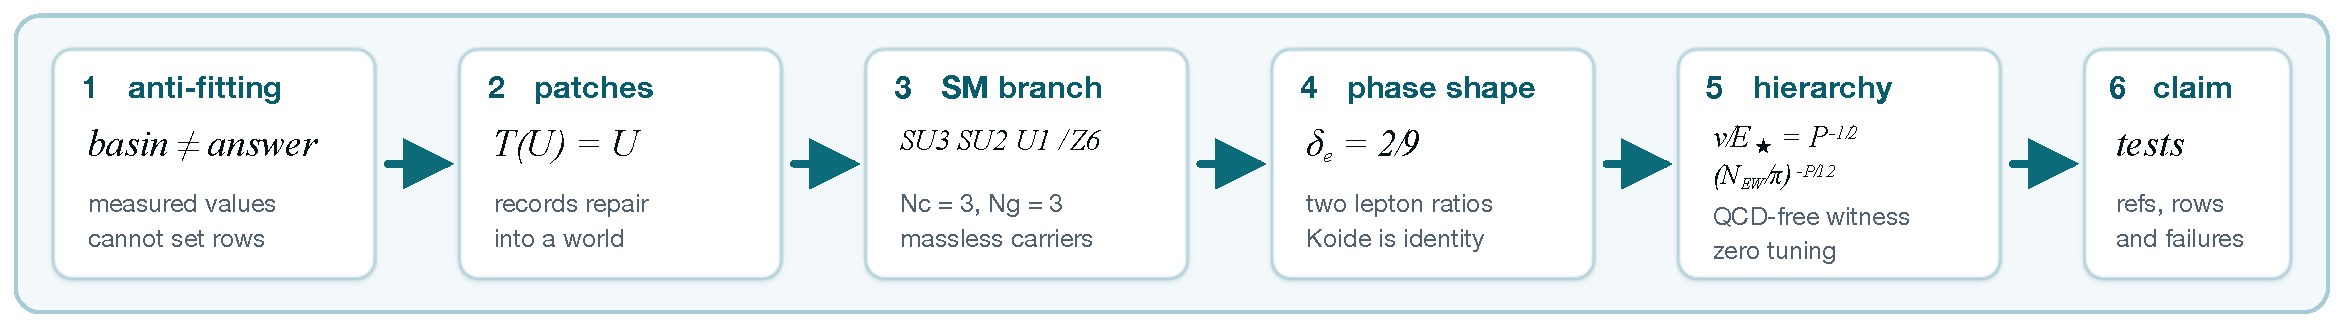
\includegraphics[width=0.93\linewidth]{assets/oph_compact_proof_spine.pdf}
\end{center}
\vspace{-0.42em}

\sect{1. The observer-patch fixed point}
The mathematical object is a finite patch system. Patches expose ports, write
records, compare overlaps, repair disagreement, and return a shared normal
form [O1,O2]. Let \(T\) be the observer-overlap repair map and let
\(\mathfrak U_{\rm OPH}\) denote the selected normal form. The simulation
identity is
\[
  T(\mathfrak U_{\rm OPH})=\mathfrak U_{\rm OPH}.
\]
The OPH simulation theorem establishes this identity from endogenous update,
observer-readable records, schedule-independent overlap repair, selected-branch
elimination, and implementation/clock closure [O2]. The universe is the stable
record world returned by its own readback-and-repair computation.

\infobox{Conditional closure theorem}{
Fix the OPH axioms, branch rules, and quotient/readout maps. Let
\[
  \Gamma_P:I_P\to I_P,
  \qquad
  \Gamma_N:I_N\to I_N
\]
be source-only contractions selected uniquely by those rules up to
observer-invisible equivalence. Banach's theorem gives unique endpoints
\[
  P_\star=\Gamma_P(P_\star),
  \qquad
  N_\star=\Gamma_N(N_\star).
\]
Every declared observable
\[
  Y_i=\pi_i\!\left(\operatorname{nf}_{\rm OPH}(P_\star,N_\star)\right)
\]
is therefore fixed by the selected branch and invariant under admissible
implementation and schedule changes. Data comparison identifies the physical
branch represented by these source outputs.}

The concrete carrier is a finite collection of local states, ports, central
records, repair maps, and checkpoints. The reference benchmark replays all six
overlap schedules and returns the same repaired normal form on the clean
abelian branches [C5]. A separate Lean\,4/Mathlib artifact certifies observer
confluence, approximate schedule independence, refinement naturality, and the
contractive conditional-resampling projector in 98 sorry-free theorems [C6].

For observer patch \(i\), the readout equations are
\[
  r_i=\mathcal R_i(\mathfrak U_{\rm OPH}),
  \qquad
  \mathfrak U_{\rm OPH}=T(\{r_i\}_{\rm compat}).
\]
The first map gives the local record; the second repairs compatible local
records into the public normal form. This is the observer-like self-reading
structure specific to OPH: local records participate in the computation that
returns the world those records describe.

\infobox{Quantum event surface}{
On a completed compare/write/verify slice, observer-accessible events generate
a finite central record algebra. For an event \(E\),
\[
  \mathbb P(E)=\operatorname{Tr}(\rho P_E),
  \qquad
  \rho|_E=\frac{P_E\rho P_E}{\operatorname{Tr}(\rho P_E)}.
\]
These are the Born rule and L\"uders update. On the associated two-wing Bell
surface,
\[
  |S_{\rm CHSH}|\le 2\sqrt2.
\]
A finite \(65{,}536\)-record run reproduces the event algebra numerically:
committed-event weights sum to \(1.0\), record projectors have zero idempotency
defect, and repeat reads are stable [O1,O3,C7].}

\sect{2. Relativity, (3+1) events, and Einstein dynamics}
The screen readout supplies an oriented conformal \(S^2\). Its connected
conformal group is the connected Lorentz group,
\[
  \mathrm{Conf}^+(S^2)
  \cong\mathrm{PSL}(2,\mathbb C)
  \cong\mathrm{SO}^+(3,1).
\]
The corresponding observer-frame space is
\[
  H^3
  \cong\frac{\mathrm{SO}^+(3,1)}{\mathrm{SO}(3)},
  \qquad
  \dim H^3=6-3=3.
\]
On the declared event branch, repaired records populate a four-dimensional
event base of signature \((-{+}{+}{+})\), while \(H^3\) is the fiber of unit
timelike observer frames over each event [O4].

The \(2\pi\)-normalized modular flow of screen caps supplies the observer-relative
clock. Half-sided modular inclusions give positive null translations; null
tomography assembles their directional charges into a conserved local
\(T_{ab}\). Fixed-cap generalized-entropy stationarity, the uniform small-ball
limit, and the all-directions tensor upgrade then compose to
\[
  G_{ab}+\Lambda g_{ab}=8\pi G_{\rm geom}\langle T_{ab}\rangle.
\]
Every arrow in this chain has a named theorem and a machine-readable receipt
type [O4,C8].

\infobox{Latest simulation receipts}{
A transactional cap-net tower with \(20/80/320\) records reaches conflict-free,
schedule-independent normal forms at every stage. On the associated Gaussian
MaxEnt collar states, the \(2\pi\)-BW profile residual improves from
\(4.4\times10^{-3}\) to \(1.1\times10^{-4}\). The realized bulk event packet
has rank four and a seed-stable ancestry cone of signature \((1,3)\), with the
modular clock aligned to its timelike direction at \(0.999\)--\(1.000\).
These are finite/one-particle witnesses for every structural receipt family in
the composed Einstein branch; the continuum result carries its declared
scaling and physical-identification receipts [O4,C7,C8].}

\sect{3. From closure coordinates to physical structure}
\vspace{0.08em}
{\bfseries\color{pragmaCyanText}The local pixel closure}\par

The source-audit pixel candidate is
\[
  P_{\rm src}=1.630972095694329\ldots .
\]
A trial pixel \(P_k\) produces a field-width readback \(R_P(P_k)\), which the
pixel chart turns into the next iterate:
\[
  \alpha_k=R_P(P_k),
  \qquad
  P_{k+1}=\Gamma_P(P_k)=\varphi+\alpha_k\sqrt\pi,
  \qquad
  \varphi=\frac{1+\sqrt5}{2}.
\]
On the selected particle branch, the internal readback chain is
\[
  P\longmapsto\alpha_U(P)\longmapsto A_Z(P)
  \longmapsto A_T^{\rm src}(P),
  \qquad
  \alpha_{\rm in}(P)=\frac{1}{A_T^{\rm src}(P)}.
\]
The intended closure equation would identify the geometric and internal readings:
\[
\begin{aligned}
  P_{\rm src}
  &=\varphi+\frac{\sqrt\pi}{A_T^{\rm src}(P_{\rm src})},\\
  \alpha_{\rm root}
  &=\frac{P_{\rm src}-\varphi}{\sqrt\pi}
   =\frac{1}{A_T^{\rm src}(P_{\rm src})}.
\end{aligned}
\]
Bisection of
\(\rho(\alpha)=\alpha_{\rm in}(\varphi+\alpha\sqrt\pi)-\alpha\)
records the candidate
\[
  \alpha_{\rm root}^{-1}=136.994835164621649\ldots .
\]
The two printed decimals have witness status. Inserting the inverse width gives
\(\varphi+\sqrt\pi/A_T^{\rm src}=1.6309720958601054\ldots\), so the printed
\(P_{\rm src}\) has residual \(-1.65776\times10^{-10}\). The
printed \(P_{\rm src}\) implies inverse width
\(136.9948369199411\ldots\). The stored source-audit status is therefore a
branch witness. A strict interval root and same-branch dependency certificate
are work in progress.
The source-audit solve is reproduced by
\[
\texttt{cd code/P\_derivation \&\& python3 derive\_p.py -{}-no-hadron-closure}.
\]
The fine-structure audit has four distinct coordinates. The source/root
witness is \(136.9948351646\ldots\), and the mixed-provenance no-hadron
diagnostic is \(137.0359595008\ldots\). An executed empirical closure using
external \(e^+e^-\to\mathrm{hadrons}\) input returns
\[
 \alpha_{\rm emp}^{-1}(0)=136.2636589431,
 \qquad
 \alpha_{\rm emp}^{-1}(0)\in
 [136.1583832834,136.3690975240].
\]
The measured endpoint is \(\alpha^{-1}(0)=137.035999177(21)\), outside that
interval. The same-scheme correction lies in
\[
[0.6485541111,0.8547920666]
\]
inverse-alpha units. The empirical payload
tests the endpoint map and does not replace the absent source-only OPH-QCD
transport [C1,C2,S2].

\vspace{0.14em}
{\bfseries\color{pragmaCyanText}The global capacity closure}\par

Let \(\Omega_N^{\rm sc}\) be the closed-screen normal forms supported at
capacity \(N\). The global source map compares their record capacity with the
screen budget and applies Minimal Admissible Realization (MAR):
\[
  S(N)=\log|\Omega_N^{\rm sc}|-N,
  \qquad
  N_\star=\operatorname{MAR}\arg\max_N S(N).
\]
The selected endpoint fixes the horizon normalization through
\[
  \Lambda_\star\ell_\star^2=\frac{3\pi}{N_\star},
  \qquad
  \Lambda_\star a_{\rm cell}=\frac{3\pi P_{\rm src}}{N_\star},
  \qquad
  a_{\rm cell}=P_{\rm src}\ell_\star^2.
\]
Thus the local loop records the candidate pair \((P_{\rm src},\alpha_{\rm root})\), while the
global loop gives the paired symbolic capacity and horizon readout
\((N_\star,\Lambda_\star)\) [O1,O4].

\vspace{0.14em}
{\bfseries\color{pragmaCyanText}The compact-gauge branch}\par

The gauge derivation starts with individually transportable seeds selected by
zero-obstruction transport. A common strict representative fixes the tensor
category carried by those seeds. Surjective pullback functors and forgetful
fibers construct its refinement limit, and Doplicher--Roberts/Tannaka
reconstruction reads off the compact group. MAR selects the realized
one-generation/one-Higgs matter package; anomaly cancellation, Yukawa
invariance, and the central kernel then fix the hypercharge lattice and quotient
[O4]. The result is
\[
  G_{\rm SM}
  =
  \frac{\mathrm{SU}(3)_c\times\mathrm{SU}(2)_L\times\mathrm{U}(1)_Y}
       {\mathbb Z_6},
  \qquad
  N_c=3,
  \qquad
  N_g=3.
\]
The selected hypercharge lattice is
\[
\begin{gathered}
  Q_i=(3,2)_{1/6},\qquad
  u_i^c=(\bar3,1)_{-2/3},\qquad
  d_i^c=(\bar3,1)_{1/3},\\
  L_i=(1,2)_{-1/2},\qquad
  e_i^c=(1,1)_1,\qquad
  H=(1,2)_{1/2},\qquad i=1,2,3.
\end{gathered}
\]
The Higgs doublet is the Borel--Weil carrier
\[
  H^0(\mathbb{CP}^1,\mathcal O(1))\cong\mathbb C^2,
  \qquad
  \operatorname{Stab}(\langle H\rangle)=\mathrm U(1)_Q.
\]
Its connected adjoint is
\[
  (8,1,0)\oplus(1,3,0)\oplus(1,1,0),
\]
which fixes charge quantization and excludes mixed \((3,2,\pm5/6)\) connected
adjoint generators. The same branch supplies the electroweak integer
\[
  \beta_{\rm EW}=N_c+1=4.
\]

\vspace{0.14em}
{\bfseries\color{pragmaCyanText}The QCD-free hierarchy witness}\par

The source-audit hierarchy witness reuses the pixel candidate and the
compact-gauge integers. Its matched unified-width coordinate is
\[
  \alpha_U(P_{\rm src})=0.04112424744557487.
\]
The screen count begins with a triangulated \(S^2\). For curvature charge
\(q_v=6-\deg(v)\), Euler's identity and \(3F=2E\) give
\[
  \sum_v q_v=6V-2E=12.
\]
Refinement-stable MaxEnt realizes the twelve units as twelve equivalent
fivefold defects, and edge-center completion turns them into twelve central
ports. Reversible write/check orientation doubles the gauge-algebra dimension:
\[
  m_{\rm rep}
  =2\dim(\mathfrak{su}(3)\oplus\mathfrak{su}(2)\oplus\mathfrak u(1))
  =2(8+3+1)=24.
\]
With local cell entropy \(\ell_{\rm cell}=P_{\rm src}/4\) and
\(\beta_{\rm EW}=4\), the electroweak share of screen depth is
\[
  \Gamma_{\rm EW}
  =\beta_{\rm EW}\ell_{\rm cell}\frac{\log(N/\pi)}{12}
  =\frac{P_{\rm src}}{12}\log(N/\pi).
\]
The corresponding transmutation law is
\[
  \frac{v}{E_\star}
  =P_{\rm src}^{-1/2}
   \exp\!\left[-\frac{2\pi}
   {\beta_{\rm EW}\alpha_U(P_{\rm src})}\right]
  =2.0198114150099223\times10^{-17}.
\]
This is the dimensionless source-audit witness.  A GeV weak scale additionally
requires an independently source-closed physical interpretation and
normalization of \(E_\star\). The exact parametric
law and the 12/24 counts are theorem outputs; the numerical endpoint has the
certificate class \texttt{source-audit branch witness} [O5,C3]. The weak scale
is a settled-form readout with naturality defect
\[
  \epsilon_H=0,
  \qquad
  \epsilon_H\in[0,0].
\]

\vspace{0.14em}
{\bfseries\color{pragmaCyanText}Conditional \(W\), \(Z\), Higgs, and top masses}\par

Once the pixel-fixed couplings and the declared electroweak surface select the
branch, the target-free value law computes the weak-boson pair with no measured
mass entering, and the downstream split relation computes the Higgs and top
coordinates on the declared running/matching/threshold surface [O5,C4]:
\[
\begin{array}{rcl}
(m_W,m_Z)_{\rm OPH} &=& (80.3770000154,\,91.1879780779)\,\mathrm{GeV},\\
(m_H,m_t)_{\rm OPH} &=& (125.1995304097,\,172.3523553288)\,\mathrm{GeV}.
\end{array}
\]
Every one of these four numbers lands on the measured value:
\begin{center}
\fontsize{7.6pt}{8.3pt}\selectfont
\setlength{\tabcolsep}{4pt}
\renewcommand{\arraystretch}{1.05}
\begin{tabular}{@{}L{0.15\linewidth}L{0.25\linewidth}L{0.27\linewidth}L{0.18\linewidth}@{}}
\toprule
\rowcolor{pragmaPanelTwo}
\textbf{Quantity} & \textbf{OPH (branch-selected)} & \textbf{Measured (PDG 2026)} & \textbf{Relative offset}\\
\midrule
\(m_W\) & \(80.3770000154\,\mathrm{GeV}\) & \(80.3692(133)\,\mathrm{GeV}\) & \(9.7\times10^{-5}\)\\
\(m_Z\) & \(91.1879780779\,\mathrm{GeV}\) & \(91.1880(20)\,\mathrm{GeV}\) & \(2.4\times10^{-7}\)\\
\(m_W/m_Z\) & \(0.8814429458\) & \(0.8813572\) & \(9.7\times10^{-5}\)\\
\(m_H\) & \(125.1995304097\,\mathrm{GeV}\) & \(125.13(11)\,\mathrm{GeV}\) & \(5.6\times10^{-4}\)\\
\(m_t\) & \(172.3523553288\,\mathrm{GeV}\) & \(172.1(6)\,\mathrm{GeV}\) & \(1.5\times10^{-3}\)\\
\bottomrule
\end{tabular}
\end{center}
The value-law pair follows as an exact implication of the five
quotient-transport premises; its finite carrier certificate (QT1--QT5) is work
in progress, so these are conditional coordinates, not physical complex-pole
masses. The Higgs/top surface carries declared calibration inputs, so that row
selects its branch and then computes the pair, inheriting the source-root,
physical-scale, running, matching, rigidity, provenance, uncertainty, and pole
gates. A diagnostic base-running chart and a target-anchored freeze-once
comparison adapter are separate audit objects, kept in the particle branch and
not shown here.

The color-amplitude/loop ansatz with
\(c=\sqrt{N_c}/2\) and \(d=N_c/2\) is a distinct conditional comparison model.
Its older four-coordinate display does not define the value law or the
declared-surface split.

\vspace{0.14em}
{\bfseries\color{pragmaCyanText}Charged-family carrier and conditional benchmark}\par

The charged-family benchmark begins with the balanced Hermitian
circulant carrier and the branch-count phase
\[
  \delta_e=\frac{\beta_{\rm EW}}{2N_cN_g}=\frac29,
  \qquad
  C_{\delta_e}
  =I+\frac{1}{\sqrt2}
  \left(e^{i\delta_e}R+e^{-i\delta_e}R^2\right),
  \qquad R^3=I.
\]
Diagonalization gives
\[
  r_k=1+\sqrt2\cos\!\left(\delta_e+\frac{2\pi k}{3}\right),
\]
and, after ordering,
\[
  (r_e,r_\mu,r_\tau)
  =(0.0403499082192,\,0.580211920148,\,2.379438171633).
\]
For \(m_i=s_e r_i^2\), the trace identities
\(\operatorname{tr}C=3\) and \(\operatorname{tr}C^2=6\) yield
\[
  \frac{\sum_i m_i}{(\sum_i\sqrt{m_i})^2}=\frac23,
\]
and the scale-free ratios are
\[
  \frac{m_\mu}{m_e}=206.770315972729\ldots,
  \qquad
  \frac{m_\tau}{m_e}=3477.47283710460\ldots .
\]
Against the PDG-2026 pole-mass summary, the two ratios differ by approximately
\(9.83\) ppm and \(30.94\) ppm [S8]. This row is a conditional retrodictive
benchmark: its stated inputs are the balanced carrier and the phase above
[O5,O6].

A separate exact geometric result begins with the screen-microphysics
icosahedron. Its twenty outward-oriented faces form \(A_5/C_3\), and each face
stabilizer cycles three corners. Every \(A_5\)-equivariantly transported
fiberwise Hermitian operator commuting with that cycle has the form
\[
  C=aI+bR+\bar bR^2,
  \qquad
  \lambda_k=a+2|b|\cos\!\left(\arg b+\frac{2\pi k}{3}\right),
\]
with a face-representative-independent unordered spectrum [O3,O5]. This exact
carrier theorem supplies the geometric three-cycle used by charged-family
source maps.

A target-informed continuation on this carrier gives
\[
 (m_e,m_\mu,m_\tau)
 =(0.510998950843394,\,105.658375501481,\,1776.930000014351)\,\mathrm{MeV}
\]
on one hybrid tuple. Its \(0.000300\)-ppm headline uses frozen rounded fields;
the tau residual is \(-1.387289\) ppm against the packet's higher-precision
central value. A conditional theorem proves that the declared
three-coordinate affine repair map is a strict contraction with one fixed
point. Source-multiplier witnesses keep the same displayed Jacobian and
contraction across different mass tuples. Evidence class: exact carrier plus a
conditional declared-map theorem. Source selection and the physical pole map
are work in progress [O5,O6].

A further conditional bridge states that a supplied chiral carrier satisfying
\(v^2\widehat Y_e\widehat Y_e^\dagger/2=J_LM_F^2J_L^\dagger\) has positive
mass response \(J_LM_FJ_L^\dagger\), and that an exact renormalized kernel with
the stipulated face-quotient Dyson readout has the same singularity operator.
The positive-square-root and determinant-zero arguments are valid. The
displayed response identity and Dyson readout are supplied physical-attachment
hypotheses; the finite model does not emit them. Its explicit zero-self-energy
kernel is a formal witness. Physical carrier selection, an interacting kernel,
and the infrared gates remain open [O5,O6].

A conditional charged face-quotient theorem states that eight stipulated
tracial registers and an exhaustive signed path packet fix the scalar affine
weights. An engineered finite model proves that this stipulated class is
nonempty. Inside a bounded patch it supplies local register state, rank-one
event readback, and a central accepted/rejected record channel
\[
 \mathcal B(H)\longrightarrow \mathcal B(H)\otimes\mathcal D_2,
 \qquad
 \mathcal D_2\cong\mathbb C\oplus\mathbb C.
\]
The evidence artifact enumerates eight register graphs, eight paths,
\(6{,}467\) matrix units, and sixty \(A_5\) charts. The register dimensions,
automaton, coupling degrees, signs, clock, and response are authored, and the
retrospective design history defeats the claimed no-target ancestry. The
checker omits some source-law and provenance fields, while its negative-control
wrapper can false-pass an unrelated nonzero exit. Schema
existence and the fixed-cutoff event-to-record bridge are proved. Physical
charged-source selection, a global recovery response, cofinal refinement,
family/Yukawa attachment, determinant normalization, coherent provenance, and
the pole scheme remain open [O5,O6].

\vspace{0.14em}
{\bfseries\color{pragmaCyanText}Common-scale quark audit}\par

The reciprocal-ray texture fails when all six inputs are written as
dimensionless Yukawas in one scheme at one scale. At \(M_Z\),
\[
 \rho_u=1.1108888543,\qquad
 \rho_d=0.7519410008,\qquad
 \rho_u\rho_d=0.8353228768,
\]
where the reciprocal law requires unit product. Granting four endpoints and
fitting the best reciprocal shape leaves a \(21.556\%\) held-out minimax error
on charm and strange. Running the common-scale audit through \(1~\mathrm{TeV}\),
\(10^5~\mathrm{GeV}\), \(10^{12}~\mathrm{GeV}\), and \(10^{16}~\mathrm{GeV}\)
leaves the same failure, with the held-out error between \(19.93\%\) and
\(21.42\%\) [O5,C2].

The exact generic physical interface is the six-scalar coordinate system
\[
 (\mu_u,\sigma_u,\rho_u,\mu_d,\sigma_d,\rho_d).
\]
The old three-scalar form is exact only inside the imposed reciprocal-ray,
affine-mean, fixed-shared-scale subfamily. Its \(0.2946\%\) and
\(0.29436\%\) residuals describe a mixed-convention retrospective chart; a
lower-order ablation reaches \(0.214229\%\) on that same chart. The particle
simulator contains no quark, Higgs, or Yukawa coupling and therefore has zero
Yukawa Fisher information. Its completed enumerated calibration is a null
result and supplies no quark-mass evidence. Generation-blind flavor-singlet scalars can
emit only the aligned \(\{I,J\}\) matrix span, leaving a physical flavor-orbit
selector absent. No nonzero source-only quark mass is emitted.

\sect{4. Geometric gravity normalization and the SI readout}
On the declared Einstein branch, the edge-entropy/area-law theorem identifies
the coefficient of the local Einstein equation
\[
  G_{ab}+\Lambda g_{ab}=8\pi G_{\rm geom}\langle T_{ab}\rangle
\]
and its Newton--Poisson limit with the observer-cell ratio
\[
  G_{\rm geom}=\frac{a_{\rm cell}}{4\bar\ell_{\rm shared}}.
\]
The local pixel branch supplies
\[
  a_{\rm cell}=P_{\rm src}\ell_\star^2,
  \qquad
  \bar\ell_{\rm shared}=\frac{P_{\rm src}}4.
\]
Substitution gives
\[
  \frac{G_{\rm geom}}{\ell_\star^2}
  =\frac{P_{\rm src}}{4(P_{\rm src}/4)}=1,
  \qquad
  \boxed{G_{\rm geom}=\ell_\star^2}.
\]
The pixel number cancels because it counts both cell area and shared edge
entropy. The factor \(4\) follows from the ratio between the structural
Einstein coefficient and the Newton--Poisson convention [O4]. This result is
the OPH normalization in geometric units.

\infobox{Newton coupling and the SI clock readout}{
A cesium clock translates the geometric identity into SI units:
\[
  \gamma_\star
  =\frac{\ell_\star\nu_{\rm Cs}}{c}
  =\frac{\varepsilon_{\rm Cs}}{2\pi},
  \qquad
  G_{\rm SI}
  =\frac{c^3\ell_\star^2}{\hbar}
  =\frac{c^5\varepsilon_{\rm Cs}^2}
  {4\pi^2\hbar\nu_{\rm Cs}^2}.
\]
For the selected display coordinate
\(\gamma_\star=4.955974336548419\ldots\times10^{-34}\), this gives
\[
  \boxed{G_{\rm SI}
  =6.674299995910528\times10^{-11}
  \,\mathrm{m^3\,kg^{-1}\,s^{-2}}}.
\]
The 2022 CODATA value is
\(6.67430(15)\times10^{-11}\,\mathrm{m^3\,kg^{-1}\,s^{-2}}\), so the display
lies \(2.7\times10^{-5}\sigma\) from its central value [S1]. Evidence class:
exact geometric normalization plus conditional SI scale/clock display. The
source-promotion certificate is the cesium record stack
\(\mathcal R_U+\mathcal R_\alpha+\mathcal R_e^{\rm abs}
+\mathcal R_{\rm QCD/nuc}^{133\rm Cs}+\mathcal R_{\rm atom}^{133\rm Cs}\)
[O1,O4,C3].}

\sect{5. Landmark solution map}
The table states the positive result first and records its evidence class once.
Paper numbers refer to the numbered OPH papers in the References block.
\begin{center}
\fontsize{7.2pt}{7.75pt}\selectfont
\setlength{\tabcolsep}{2.4pt}
\renewcommand{\arraystretch}{0.98}
\begin{longtable}{@{}L{0.18\linewidth}L{0.55\linewidth}L{0.16\linewidth}L{0.07\linewidth}@{}}
\toprule
\rowcolor{pragmaPanelTwo}
\textbf{Physics problem} & \textbf{OPH solution on the declared branch} & \textbf{Evidence class} & \textbf{Paper}\\
\midrule
\endhead
Observer and measurement problem &
An observer is a bounded self-reading record boundary. Compatible local
readouts participate in the repair map that returns the public world
\(T(\mathfrak U)=\mathfrak U\). & Internal theorem & 1,2\\

Quantum probabilities and update &
The finite central record algebra yields the Born rule, L\"uders conditioning,
and \(|S_{\rm CHSH}|\le2\sqrt2\) on the two-wing event surface. &
Internal theorem & 1,3\\

Time, Lorentz symmetry, and three space dimensions &
Cap modular flow supplies the relative clock;
\(\mathrm{Conf}^+(S^2)\cong\mathrm{SO}^+(3,1)\), and
\(H^3\cong\mathrm{SO}^+(3,1)/\mathrm{SO}(3)\) has dimension three over a
\(3+1\) event base. & Receipt-conditional theorem & 4\\

General relativity &
Null translations, local stress, generalized-entropy stationarity, and the
uniform small-ball limit compose to
\(G_{ab}+\Lambda g_{ab}=8\pi G\langle T_{ab}\rangle\). &
Receipt-conditional theorem & 4\\

Gravity from quantum information &
The edge-entropy/area law fixes the Einstein and Newton coefficient:
\(G_{\rm geom}=a_{\rm cell}/(4\bar\ell_{\rm shared})=\ell_\star^2\). &
Internal identity & 4\\

Standard Model gauge and matter structure &
DR/Tannaka reconstruction plus MAR, anomaly cancellation, and Yukawa
invariance give
\((\mathrm{SU}(3)\times\mathrm{SU}(2)\times\mathrm{U}(1))/\mathbb Z_6\),
the hypercharge lattice, \(N_c=N_g=3\), and one Higgs doublet. &
Realized-branch theorem & 4\\

Electroweak breaking and charge quantization &
The Borel--Weil Higgs carrier
\(H^0(\mathbb{CP}^1,\mathcal O(1))\cong\mathbb C^2\) has stabilizer
\(\mathrm U(1)_Q\); the connected adjoint fixes the Standard Model charge
lattice. & Realized-branch theorem & 4\\

Electroweak and Higgs mass scale &
Branch selection fixes the electroweak surface, and the target-free value law
computes \((m_W,m_Z)=(80.377,91.188)\,\mathrm{GeV}\) to \(10^{-4}\) of
measurement; the declared-surface split gives
\((m_H,m_t)=(125.20,172.35)\,\mathrm{GeV}\). No promoted complex-pole mass. &
Conditional target-free chart + declared-surface split & 5\\

Electromagnetism and force carriers &
The unbroken \(\mathrm U(1)_Q\) branch fixes the electromagnetic connection.
With the declared quadratic actions, Maxwell has two transverse modes,
perturbative Yang--Mills has \(2\dim G\), and Einstein gravity has two
transverse-traceless modes. & Conditional action theorem & 1,4\\

Proton stability &
The selected product-group gauge structure contains no grand-unified gauge
bosons connecting quarks to leptons and therefore excludes gauge-mediated
proton decay on the realized branch. & Realized-branch corollary & 1,4\\

Weak/UV hierarchy and Higgs naturality &
The 12-port screen, 24-slot oriented register, \(P_{\rm src}\), and
\(\alpha_U(P_{\rm src})\) emit \(v/E_\star\sim2.02\times10^{-17}\) with
\(\epsilon_H=0\). & Source-audit witness & 5\\

Fine-structure source scale &
The source/root witness, mixed diagnostic, empirical external-data endpoint,
and measured endpoint are distinct. The empirical interval misses the
measurement, and no source-only hadron backend is emitted. &
Source witness + empirical audit & 5,6\\

Dark energy / cosmological term &
The global record-capacity closure fixes
\(\Lambda_\star\ell_\star^2=3\pi/N_\star\), while vacuum energy lies in the
kernel of the local null readout. & Symbolic closure theorem & 1,4\\

Dark-matter phenomenology &
Repair-stress bookkeeping gives the galaxy continuation
\(\nu_{\rm OPH}(x)=[1-e^{-\lambda_{\rm collar}\sqrt x}]^{-1}\) and the deep
limit \(v^4=GM_ba_{\rm eff}\). & Conditional continuation & 7\\

Yang--Mills gap &
On the controlled compact-gauge continuum branch, the transfer/repair theorem
identifies \(\Delta_{\rm YM}=\Delta_{\rm rep}>0\). &
Conditional theorem & 8\\

Family geometry &
The icosahedral face bundle \(A_5/C_3\) gives an exact local cyclic carrier;
the charged continuation is target-anchored, and the finite face-quotient
model proves fixed-cutoff schema existence. No nonzero source-only physical
mass is emitted. & Exact carrier + conditional map & 3,5,6\\

String-vacuum selection &
Observer-patch consistency defines a finite sieve over critical-string
candidates; the Bouchard--Donagi geometry is selected on its declared gate
stack. & Conditional selection program & 9\\
\bottomrule
\end{longtable}
\end{center}

\sect{6. Best quantitative outputs and checks}
\begin{center}
\fontsize{7.15pt}{7.55pt}\selectfont
\setlength{\tabcolsep}{2.8pt}
\renewcommand{\arraystretch}{0.98}
\begin{longtable}{@{}L{0.20\linewidth}L{0.20\linewidth}L{0.43\linewidth}L{0.11\linewidth}@{}}
\toprule
\rowcolor{pragmaPanelTwo}
\textbf{Output} & \textbf{Evidence class} & \textbf{Value and check} & \textbf{Paper / receipt}\\
\midrule
\endhead
Finite observer-patch normal form &
Internal theorem &
All six overlap schedules return the same repaired normal form on the clean
abelian branches, with zero schedule divergence. &
1,2 / C5\\

Quantum event surface &
Internal theorem &
On \(65{,}536\) records, Born weights sum to \(1.0\), projector idempotency
defect is zero, and repeat-read fraction is \(1.0\); analytically
\(|S_{\rm CHSH}|\le2\sqrt2\). &
1,3 / C7\\

Lorentz and Einstein chain &
Receipt-conditional theorem &
BW residual improves \(4.4\times10^{-3}\to1.1\times10^{-4}\); the realized
bulk packet has rank four, signature \((1,3)\), and clock alignment
\(0.999\)--\(1.000\). &
4 / C8\\

Standard Model branch &
Receipt-conditional realized theorem &
Exact quotient \(\mathbb Z_6\), one Higgs doublet, and
\((N_c,N_g,\beta_{\rm EW})=(3,3,4)\), matching the observed discrete
architecture. &
4\\

Classical force content &
Conditional action theorem &
Two transverse Maxwell modes, \(2\dim G\) perturbative pure-Yang--Mills
modes, and two transverse-traceless Einstein modes, all with the common
massless quadratic kernel on their declared action branches. &
1,4\\

Source electromagnetic root &
Source-audit numerical witness &
\(P_{\rm src}=1.630972095694329\ldots\) and
\(\alpha_{\rm root}^{-1}=136.994835164621649\ldots\); the source-to-CODATA
relative offset is \(3.00\times10^{-4}\). &
5,6 / C1\\

EW-refined capacity &
Public-endpoint bridge fixed point &
\(N_{\rm CRC}^{\rm EW}=3.5323546226929907\times10^{122}\); its logarithmic
depth differs from the rounded \(3.31\times10^{122}\) de Sitter scale by
\(2.1\times10^{-4}\). &
5 / C3\\

Weak hierarchy &
Source-audit numerical witness &
\(\alpha_U(P_{\rm src})=0.04112424744557487\) and
\(v/E_\star=2.0198114150099223\times10^{-17}\), with \(\epsilon_H=0\). &
5 / C3\\

\(W\), \(Z\), Higgs, top masses &
Target-free value law + conditional split &
The target-free value law computes \((m_W,m_Z)=(80.377,91.188)\,\mathrm{GeV}\)
within \(10^{-4}\) of measurement with no fitted mass; the declared-surface
split gives \((m_H,m_t)=(125.20,172.35)\,\mathrm{GeV}\) within
\(1.5\times10^{-3}\). No promoted complex-pole mass. &
5 / C4\\

Charged-family geometry &
Exact carrier + conditional declared-map theorem &
The \(A_5/C_3\) face bundle gives local cyclic fibers, and the engineered
finite model connects noncentral events to central records at fixed cutoff.
No nonzero source-only physical mass is emitted. &
3,5,6\\

Geometric gravity &
Internal identity &
The cell-area/shared-entropy theorem gives the exact normalization
\(G_{\rm geom}/\ell_\star^2=1\). &
4\\

SI gravity readout &
Conditional scale/clock display &
\(G_{\rm SI}=6.674299995910528\times10^{-11}\) in SI units, lying
\(2.7\times10^{-5}\sigma\) from the CODATA central value. &
1,4 / S1\\

Galaxy scorecard &
Conditional galaxy continuation &
SPARC \(\chi^2/{\rm point}=1.017\), velocity RMS
\(11.25\,\mathrm{km\,s^{-1}}\), and RAR scatter \(0.13\) dex; same-function
reference \(\chi^2/{\rm point}=1.023\). &
7 / C9\\
\bottomrule
\end{longtable}
\end{center}

\sect{7. Why coincidence is unlikely}
\infobox{One source, every major layer}{
One finite self-reading architecture reaches quantum theory, \(3+1\) spacetime,
Einstein gravity, the Standard Model, the weak hierarchy, cosmic closure, and
Newton normalization. Sector-specific fitted decimals in this core: \(0\).}

\begin{center}
\fontsize{7.8pt}{8.45pt}\selectfont
\setlength{\tabcolsep}{3pt}
\renewcommand{\arraystretch}{1.07}
\begin{tabular}{@{}L{0.62\linewidth}L{0.22\linewidth}L{0.10\linewidth}@{}}
\toprule
\rowcolor{pragmaPanelTwo}
\textbf{Core event} & \textbf{Generous window} & \textbf{Factor}\\
\midrule
The same patch rules support Lorentz \(3+1\) kinematics and the Einstein chain &
one chance in ten & \(10^{-1}\)\\
The realized compact branch lands on the exact Standard Model quotient,
hypercharge/matter lattice, three colors, and three generations &
one chance in one thousand & \(10^{-3}\)\\
The electromagnetic source/root value remains a branch witness. Its strict
dependency certificate is absent, and the empirical external-data closure
misses the measured endpoint & excluded from this score & \(1\)\\
The same electroweak branch lands the \(10^{-17}\) hierarchy exponent
(\(\epsilon_H=0\)) and computes the target-free \(W/Z\) value law to
\(10^{-4}\) of measurement & one chance in one thousand & \(10^{-3}\)\\
\bottomrule
\end{tabular}
\end{center}

\[
  p_{\rm coincidence}
  =(10^{-1})(10^{-3})(1)(10^{-3})
  =10^{-7},
  \qquad
  -\log_2p_{\rm coincidence}=23.3\ \text{bits}.
\]
Give OPH and coincidence equal odds before reading the table, use the product
as the likelihood of the evidence under coincidence, and apply a \(10^4\)
search penalty. The simple Bayes score is
\[
 \boxed{\Pr(\text{OPH incorrect}\mid E)
 \approx\frac{10^4p_{\rm coincidence}}
 {1+10^4p_{\rm coincidence}}
 =0.0999\%},
\]
about one chance in 1001. A calibrated posterior would require measured
likelihoods and a defensible prior; this score keeps its assumptions visible.

\vspace{-0.08em}
\sect{References}
{\fontsize{7.1pt}{7.75pt}\selectfont
\setlength{\columnsep}{1.2em}
\begin{multicols}{2}
\raggedcolumns
\textbf{Data and standards}
\refentry{[S1]}{CODATA Task Group (2024). ``2022 CODATA recommended values:
Newtonian constant of gravitation.'' \href{https://physics.nist.gov/cuu/pdf/wall_2022.pdf}{NIST Reference on Constants}.}
\refentry{[S2]}{CODATA Task Group (2024). ``2022 CODATA recommended values:
inverse fine-structure constant.'' \href{https://physics.nist.gov/cuu/pdf/wall_2022.pdf}{NIST Reference on Constants}.}
\refentry{[S8]}{Particle Data Group (2026). ``Leptons.''
\href{https://pdg.lbl.gov/2026/tables/rpp2026-sum-leptons.pdf}{Review of Particle Physics summary table}.}

\textbf{OPH papers}
All OPH series papers below use release \texttt{\OPHPaperReleaseID}.
\refentry{[1/O1]}{Mueller et al. (2026). \href{https://github.com/FloatingPragma/observer-patch-holography/blob/main/paper/observers_are_all_you_need.tex}{``Observers Are All You Need.''}}
\refentry{[2/O2]}{M\"uller et al. (2026). \href{https://github.com/FloatingPragma/observer-patch-holography/blob/main/paper/reality_as_consensus_protocol.tex}{``Reality as a Consensus Protocol: The Fixed-Point Computation That Implements Physics.''}}
\refentry{[3/O3]}{M\"uller et al. (2026). \href{https://github.com/FloatingPragma/observer-patch-holography/blob/main/paper/screen_microphysics_and_observer_synchronization.tex}{``Federated Echosahedral Screen Microphysics: Patch Hardware, Records, and Observer Synchronization in OPH.''}}
\refentry{[4/O4]}{M\"uller et al. (2026). \href{https://github.com/FloatingPragma/observer-patch-holography/blob/main/paper/recovering_relativity_and_standard_model_structure_from_observer_overlap_consistency_compact.tex}{``Recovering Relativity and the Standard Model from Observer Overlap Consistency.''}}
\refentry{[5/O5]}{M\"uller et al. (2026). \href{https://github.com/FloatingPragma/observer-patch-holography/blob/main/paper/deriving_the_particle_zoo_from_observer_consistency.tex}{``Deriving the Particle Zoo from Observer Consistency.''}}
\refentry{[6/O6]}{M\"uller, B. (2026). \href{https://github.com/FloatingPragma/observer-patch-holography/blob/main/extra/fine_structure_constant_derivation.tex}{``The Fine-Structure Constant as an OPH Pixel Fixed Point.''} OPH technical note.}
\refentry{[7/O7]}{Mueller, B., and D. Matscheko (2026). \href{https://github.com/FloatingPragma/observer-patch-holography/blob/main/cosmology/oph_dark_matter_paper.tex}{``Observer-Patch Holography and the Dark Matter Phenomenon.''}}
\refentry{[8/O8]}{M\"uller, B. (2026). \href{https://github.com/FloatingPragma/observer-patch-holography/blob/main/extra/yang_mills_gap_clay_problem.tex}{``Explaining the Yang--Mills Mass Gap with Observer-Patch Repair Dynamics.''} OPH technical note.}
\refentry{[9/O9]}{M\"uller, B. (2026). \href{https://github.com/FloatingPragma/observer-patch-holography/blob/main/extra/observer_patch_holography_as_string_vacuum_selector.tex}{``Observer-Patch Holography as a String-Vacuum Selector.''} OPH technical note.}

\textbf{Executable artifacts}
\refentry{[C1]}{FloatingPragma (2026). \href{https://github.com/FloatingPragma/observer-patch-holography/tree/main/code/P_derivation}{Pixel-closure solver and receipts}.}
\refentry{[C2]}{FloatingPragma (2026). \href{https://github.com/FloatingPragma/observer-patch-holography/tree/main/code/particles}{Particle-branch source and audit suite}.}
\refentry{[C3]}{FloatingPragma (2026). \href{https://github.com/FloatingPragma/observer-patch-holography/tree/main/code/particles/hierarchy}{Hierarchy theorem package and receipts}.}
\refentry{[C4]}{FloatingPragma (2026). \href{https://github.com/FloatingPragma/observer-patch-holography/tree/main/code/particles/runs/calibration}{Electroweak calibration receipts}.}
\refentry{[C5]}{FloatingPragma (2026). \href{https://github.com/FloatingPragma/observer-patch-holography/tree/main/code/consensus}{Consensus schedule benchmarks}.}
\refentry{[C6]}{FloatingPragma (2026). \href{https://github.com/FloatingPragma/observer-patch-holography/tree/main/Lean}{Lean 4/Mathlib theorem artifact}.}
\refentry{[C7]}{Mueller, B. (2026). \href{https://github.com/muellerberndt/oph-physics-sim}{OPH-FPE simulation and receipts, including the quantum-record, BW/KMS, \(H^3\), and geometry runs}.}
\refentry{[C8]}{FloatingPragma (2026). \href{https://github.com/FloatingPragma/observer-patch-holography/tree/main/code/geometry}{Lorentz--Einstein geometry receipts}.}
\refentry{[C9]}{FloatingPragma (2026). \href{https://github.com/FloatingPragma/observer-patch-holography/tree/main/code/dark_matter}{SPARC galaxy scorecard and receipts}.}
\end{multicols}
}

\end{document}
